%% Mark to describe method used to tag and time articles 
\documentclass[a4paper, 12pt]{article} 
\usepackage{amsmath, amssymb, color, graphicx, enumitem}
\usepackage{fullpage} %smaller margins
\usepackage{hyperref} % hyperlinks
\usepackage{url} %sensible urls
\usepackage{todo} %creates todo in margins
\usepackage{booktabs} % better looking tables


%font, libertine
\usepackage{libertine}
%word spacing
\usepackage{microtype}
%all equations get full space
\everymath{\displaystyle}

%columns separate and line
\usepackage{multicol}
\setlength{\columnsep}{1.5cm}
\setlength{\columnseprule}{0.2pt}

%environment
\newcommand{\tab}{\phantom{ssss}}

%=======================Shortcuts==============================================
%useful shortcuts
\def\R{\ensuremath{\mathbb{R}}} %\ensuremath adds math mode, if forgotten
\def\Q{\ensuremath{\mathbb{Q}}}
\def\N{\ensuremath{\mathbb{N}}}
\def\Z{\ensuremath{\mathbb{Z}}}
\def\C{\ensuremath{\mathbb{C}}}

%shorcuts with arguments
\newcommand{\abs}[1]{\left\vert#1\right\vert} %nice absolute values
\newcommand{\bt}[1]{\textbf{#1}} %bold
\newcommand{\eq}[1]{\begin{align*}#1\end{align*}} %aligned equations
\newcommand{\norm}[1]{\left\lVert#1\right\rVert} %vector norm
\newcommand{\notimplies}{% does not imply
    \mathrel{{\ooalign{\hidewidth$\not\phantom{=}$\hidewidth\cr$\implies$}}}}
\renewcommand{\eq}[1]{\begin{align*}#1\end{align*}} %aligned equations


%colors
\definecolor{javagreen}{rgb}{0.25,0.5,0.35} %dark green color
\definecolor{lightblue}{rgb}{0.149,0.545,0.824} %solarized blue
\definecolor{sred}{rgb}{0.863, 0.196, 0.184} %solarized red

\newcommand{\blue}[1]{{\leavevmode\color{lightblue}{#1}}} %solarized blue 
\newcommand{\green}[1]{{\leavevmode\color{javagreen}{#1}}} %command for green
\newcommand{\red}[1]{{\leavevmode\color{sred}{#1}}} %solarized red
\newcommand{\gray}[1]{{\leavevmode\color[gray]{0.5}{#1}}} %gray text

%==TODO==
% boxes?
%checkout: http://blog.rtwilson.com/my-latex-preamble/

\title{}
\date{}
% ========================== Tips =============================================
%part
    %section, sub, sub

%\begin{enumerate}[resume] %continues counting

% Piecewise Function
%\begin{displaymath}
%   f(x) = \left\{
%     \begin{array}{lr}
%       1 & : x \in \mathbb{Q}\\
%       0 & : x \notin \mathbb{Q}
%     \end{array}
%   \right.
%\end{displaymath} 

% Images
% \includesgraphics{image.png}

% Tables
%\begin{tabular}{llr}
%    \toprule
%    first name & last name & $\chi$\\
%    \midrule
%    second & last & first \\
%    \bottomrule
%\end{tabular}

% ========================== End of Tips ======================================

% figures path
\graphicspath{{figures/}}

\begin{document}
\begin{center}
\section*{Intro and Methods}
\end{center}


\subsection*{Notes}

Categories, third level.
    * total is 235,000 entry categories
* The Thesaurus was compiled over a period of 44 years
* While the OED is a hugely rich resource for studying the histories of individual words, there was no parallel resource for studying the history of concepts as they are expressed in word
* classificatory principle on which the Thesaurus is based: a progression from the most general terms to the most specific.
* from editor notes: "A scroll through a section such as Food or Inhabiting/dwelling illustrates how far people’s lives have changed over time."


\subsection*{Introduction}

* topic modelling is a huge area of research (complicated methods exist, but not perfect)
* we introduce a simple mechanism to tag articles (and vary the granularity of cateogries) 
    * this approach provides the additional benefit of zooming back in time
        * what would the text have looked like using vocabulary of an earlier time.
* we use Wikipedia as a dataset 
    * encompasses a variety of topics, which fit into many categories
    * edited by many authors (no bias from a single author's writing)
    * provides a large body of text on which to demonstrate the method


\subsection*{Historical Thesaurus}

While the Oxford English Dictionary is one of the richest sources of information about individual words, it does not provide a way to parse the hierarchical relationships among them.
The Historical Thesaurus is a categorical hierarchy of the English Language based on the OED and compiled over 44 years
[cite historical thesaurus site]. 
The Historical Thesaurus spans the history of the English language from Old English (~1000 AD) to
the year 2000 and contains nearly $800,000$ words.
The authors placed each word into a category based on the word's definition and synonyms.


The authors organized words into several category levels with a total of $235,000$ categories. At the highest level are three categories:
the world, the mind, and society. 
The second level provides subcategories for each category in the highest level, branching the highest level into 37 categories. 
For example, underneath the world are categories such as life and space. 
At level three there are $377$ categories and at level 4 there are $1,927$. 
Since words can have more than one definition or sense, some subcategories appear under multiple categories.
[add example]
Furthermore, some categories into up to seven levels, although the tree is incomplete: 
some categories only branch out into three or four levels, while others into seven.



\subsection*{Tagging Topics}

This hierarchical organization of words into categories provides as its authors say, 
"a rich resource for studying the history of concepts as they are expressed in word."
More than definitions, this data set provides a systematic means to extract topic categories with 
a varying level of detail for a piece of text. We propose a tagging method to automatically identify the categories of a particular text.

Given a piece of text, we first identify word the words using standard NLP methods 
(removing punctuation, using spaces as delimiters etc.). Then, we identify the categories at a particular 
level each word belongs to. If we're interested a detailed categorization, we might use level three or four categories, for a more coarse categorization we may use say level two.
We increment the count of each category by the number of words in the text.  
If ten words belong to "Parts of a Clock", then "Parts of a Clock" receives a weight of 10.
See figure below:


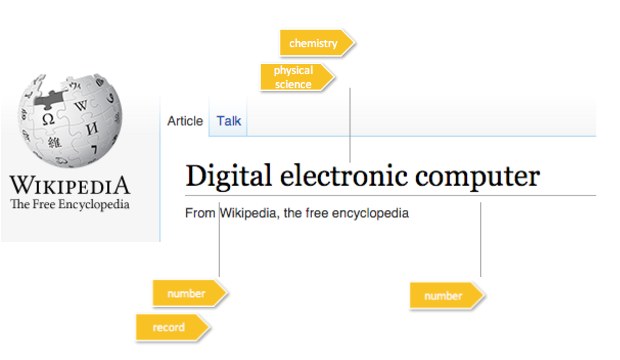
\includegraphics[width=\textwidth]{title_tags}  

In addition to incremented category tags, we also tag each word with the date of its earlier appearance in 
the OED. This allows us to identify the date of the words used to express concepts in a particular category.
Consequently, we can zoom back in time, by eliminating words with a date of appearance that is after
a particular date of interest.

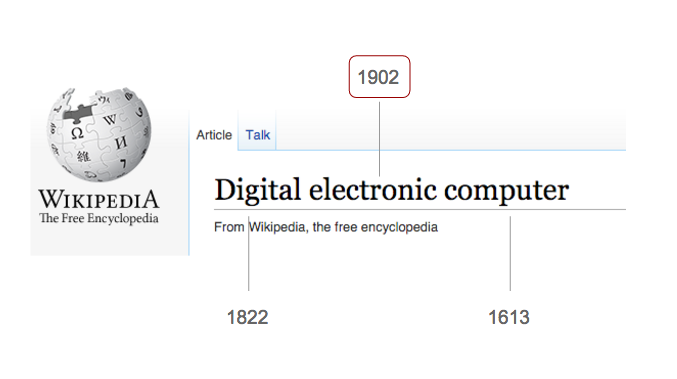
\includegraphics[width=\textwidth]{title_dates}  


While we are able to sysmetically obtain a list of categories with corresponding weights for a given 
piece of text, we note that this method does not distinguish between different senses of a word. 
Instead, a word with multiple sense will yield multiple categories. The date used to tag a word is the 
date of the earlier appearance of any of the possible senses of a word.


\subsection*{Application to Wikipedia}

To illustrate how the technique works, we apply this tagging method to the dataset of all 
5 million English Wikipedia articles  as of November, 2014. 
We use the title of each article as the input text to tag each with categories and a date.
As outlined above, we tag each article with categories based on categories in which each word 
belongs in the historical thesaurus. 
We use the third level categories, because it strikes a balance between being too coarse 
yet not useful and too fine as to be overwhelming. 
This enables us to tag each article with up to 377 distinct categories. Furthermore, 
we tag each article with a date, which captures the earliest year in which the words
in the title would have been in usage. 

By tagging articles with a date and category, we can identify o
* cateogries of knowledge
* historical zoom through

as use this idea not only to tag categories to obtain a view of the areas of knowledge through article titles, 
but we also obtain a historical pesepctive of wikipedia.


\subsection*{Style Guide}

\begin{itemize}
    \item  tag or category? 
        \begin{itemize}
            \item  tag a text with a category?
        \end{itemize}
    \item  should we use quotes for category names or bold face as Fletcher did in his thesis?
\end{itemize}

\end{document}

